\documentclass{article}
\usepackage[utf8]{inputenc}
\usepackage[margin = 0.8in]{geometry}
\usepackage{graphicx}
\usepackage{amsmath, amssymb}
\usepackage{subcaption}
\usepackage{multirow}
\usepackage{mathtools}
\usepackage{float}


\title{RBE595 - Week 3 Assignment}
\author{Keith Chester}
\date{Due date: January 30, 2023}

\begin{document}
\maketitle

\section*{Problem 1}
\textit{Suppose $\gamma = 0.8$ and we get the following sequence of rewards $R_1 = -2$ , $R_2 = 1$ , $R_3 = 3$ , $R_4 = 4$, $R_5 = 1.0$
    Calculate the value of $G_0$ by using the equation 3.8 (work forward) and 3.9 (work backward) and show they yield the same results. }

Utilizing the equation:

\begin{equation}
    G_t = \sum_{k=0}^{\infty} \gamma^k R_{t+k+1}
\end{equation}

...and our sequence of rewards, we can calculate moving forwards:

\begin{equation}
    G_0 = \gamma^0 R_1 + \gamma^1 R_2 + \gamma^2 R_3 + \gamma^3 R_4 + \gamma^4 R_5
\end{equation}

\begin{equation}
    G_0 = 0.8^0 * -2 + 0.8^1 1 + 0.8^2 3 + 0.8^3 4 + 0.8^4 1
\end{equation}

\begin{equation}
    G_0 = 1 * -2 + .8 * 1 + .64 * 3 + .512 * 4 + .4096 * 1 = 3.1776
\end{equation}

...and then to show that it's the same when working backwards:

\begin{equation}
    G_t = R_{t+1} + \gamma G_{t+1}
\end{equation}

...and working backwards, with $G_5=0$:

\begin{equation}
    G_4 = R_5 + \gamma G_5 = 1 + 0.8 * 0 = 1
\end{equation}

\begin{equation}
    G_3 = R_4 + \gamma G_4 = 4 + 0.8 * 1 = 4.8
\end{equation}

\begin{equation}
    G_2 = R_3 + \gamma G_3 = 3 + 0.8 * 4.8 = 6.84
\end{equation}

\begin{equation}
    G_1 = R_2 + \gamma G_2 = 1 + 0.8 * 6.84 = 6.472
\end{equation}

\begin{equation}
    G_0 = R_1 + \gamma G_1 = -2 + 0.8 * 6.472 = 3.1776
\end{equation}


\section*{Problem 2}

\textit{Explain how a room temperature control system can be modeled as an MDP? What are the states, actions, rewards, and transitions.}

\begin{itemize}
    \item \textbf{States} - The temperature controller state is the error difference between a stated desired temperature and the current temperature read from its sensor(s).
    \item \textbf{Actions} - Assuming a rudimentary on/off control which most housing AC and heaters are, the temperature controller can perform three actions - heat (heater on, AC off), cool (AC on, heater off), and off (both heater and AC is off).
    \item \textbf{Rewards} - The temperature controller is rewarded by keeping the difference between the target temperature ($T_t$) and the current temperature ($T_c$). Since we are trying to produce an agent that *maximizes* the reward, we would want to mathematically change the difference such that the lower the difference, the higher our reward. Thus we'll try something like $1 + | T_t - T_c |$. You could also use $\frac{1}{|T_c-T_C|}$ but would have to deal with $T_t = T_c$ making this reward undefined.
    \item \textbf{Transitions} - Transitions between states would be a resulting temperature change. A time step would be some amount of time for reasonable change to occur (ie in a room temperature controller, several minutes. In a liquid bath temperature controller, maybe 30 seconds).
\end{itemize}

\section*{Problem 3}

\textit{What is the reward hypothesis in RL?}

The reward hypothesis is an expression that all that we discuss and encompass with goals, rewards, and purposes of the agent is ultimately a representative scalar value that the agent, in turn, is attempting to maximize. Specifically the culmultative reward, not immediate per-action rewards.

\section*{Problem 4}

\textit{We have an agent in maze-like world. We want the agent to find the goal as soon as possible. We set the reward for reaching the goal equal to +1 With $\gamma$ = 1. But we notice that the agent does not always reach the goal as soon as possible. How can we fix this?}

$\gamma$ represents a discount rate, from which we discount the value of future rewards, calculated via:

\begin{equation}
    G_t = \sum_{k=0}^{\infty} \gamma^k R_{t+k+1}
\end{equation}

By utilizing $\gamma=1$, we are essentially not applying any discount to future reward values at all, thus not providing any form of a penalty against longer courses of actions that still result in the same reward. If we decrease $\gamma$ to a value $0 > \gamma < 1$, we would begin to push the agent to favor quicker courses of actions towards its goal.

\section*{Problem 5}

\textit{What is the difference between policy and action?}

An action is an option that an agent can take in a given state. An agent's policies maps the actions to a set of probabilities that the agent will choose that action for that given state.

\section*{Problem 6}

\textit{Exercise 3.14 from the book: The Bellman equation (3.14) must hold for each state for the value function $v_\pi$ shown in Figure 3.2 (right) of Example 3.5. Show numerically that this equation holds for the center state, valued at $+0.7$, with respect to its four neighboring states, valued at $+2.3$, $+0.4$, $-0.4$, and $+0.7$. (These numbers are accurate only to one decimal place)}

Here we aim to calculate the Bellman equation to show that its value is equal to our cener value.

\begin{equation}
    v_\pi (s) = \sum_a \pi(a|s) \sum_{s',r} p(s',r|s,a) \bigl( r+\gamma v_\pi (s') \bigr)
\end{equation}

\begin{equation}
    v_\pi (s) = 0.25*(0+0.9*2.3)+0.25* (0 + 0.9 * 0.4) + 0.25*(0+ 0.9*-0.4) + 0.25*(0+0.9*0.7)
\end{equation}

\begin{equation}
    v_\pi (s) = 0.7
\end{equation}

\noindent ...and this matches the center value as we set out to show.

\section*{Problem 7}

\textit{Exercise 3.17 from the book: What is the Bellman equation for action values, that is, for $q_\pi$? It must give the action value $q_\pi ( s, a )$ in terms of the action values, $q_\pi ( s' , a' )$, of possible successors to the state–action pair $( s, a )$. Hint: the backup diagram to the right corresponds to this equation.Show the sequence of equations analogous to (3.14), but for action values.}

First, let us express $q_\pi (s, a)$:

\begin{equation}
    q_\pi (s,a) = E_\pi \big[ G_t | S_t = s, A_t = a \big]
\end{equation}

\noindent The book's equation 3.13 allows us to expand on this:

\begin{equation}
    q_\pi(s,a) = E_\pi \big[ \sum^\infty_{k=0} \gamma^k r_{t+k+1} | S_t = s,A_t =a \big]
\end{equation}

\noindent From this we can pull out the first reward of the equation:

\begin{equation}
    q_\pi(s,a) = E_\pi \big[ r_{t+1} + \gamma \sum^\infty_{k=0} \gamma^k r_{t+k+2} | S_t = s,A_t =a \big]
\end{equation}

\begin{equation}
    q_\pi(s,a) = E_\pi \big[ r_{t+1} | S_t=s, A_t=a \big] + E_\pi \big[ \gamma \sum^\infty_{k=0} \gamma^k r_{t+k+2} | S_t = s,A_t =a \big]
\end{equation}

\begin{equation}
    q_\pi(s,a) = \sum_{s',r} p(s',r|s,a) r(s,a,s') +
    \gamma E_\pi \big[ G_t | S_t=s, A_t=a \big]
\end{equation}

\begin{equation}
    q_\pi(s,a) = \sum_{s'} p(s',|r|s,a)r(s,a,s')+
    \sum_{s',r} p(s',r|s,a) \gamma \sum_{a'} \pi(s',a') E_\pi \big[
    G_{t+1}|S_{t+1}=s',A_{t+1}=a'
    \big]
\end{equation}

Remember, that we stated before that $q_\pi(s,a) = E_\pi \big[ G_t | S_t = s, A_t = a \big]$ - extending that to $q_\pi(s',a')$, we get $q_\pi(s',a') = E_\pi \big[ G_t | S_t = s', A_t = a' \big]$ and subsibtute accordingly, leading us to:

\begin{equation}
    q_\pi (s,a) = \sum_{s',r} p(s',r|s,a) \big[
        r(s,a,s')+\gamma \sum_{a'} \pi(a'|s')q(s',a')
        \big]
\end{equation}


\section*{Problem 8}

\textit{Exercise 3.22 from the book: Consider the continuing MDP shown below. The only decision to be made is that in the top state, where two actions are available, left and right. The numbers show the rewards that are received deterministically after each action. There are exactly two deterministic policies, left and right. What policy is optimal if $\gamma = 0$? If $\gamma = 0.9$? If $\gamma = 0.5$?}

\begin{figure}[H]
    \centering
    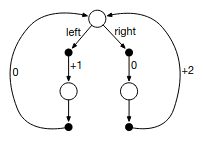
\includegraphics[width = 0.45\textwidth]{imgs/exercise_8.png}
    \caption{MDP For Problem 8}
    \label{fig:exercise8}
\end{figure}

First, we look at the equation for a given policy $q_\pi$, such that:

\begin{equation}
    q_\pi(s,a) = \sum_a p(s',r|s,a)+\gamma \sum_{s',r} \pi(a'|s')q(s'|a')
\end{equation}

\noindent Our problem states that the policy is deterministic, thus we can modify the above function and simplify it to the following functions for each possible action, starting with our right:

\begin{equation}
    q_\pi(s,right) = \sum_a p(s',r|s,right)r + \gamma \sum_{s',r} \pi(a'|s')q(s',a') = 1 * 0 + \gamma * 2 = 2\gamma
\end{equation}

\noindent ...and our left:

\begin{equation}
    q_\pi(s,left) = \sum_a p(s',r|s,left)r + \gamma \sum_{s',r} \pi(a'|s')q(s',a') = 1 * 1 + \gamma * 0 = 1
\end{equation}

With this in mind, the question wishes us to explore what would happen given a value of $\gamma$:

\begin{itemize}
    \item \textbf{$\gamma=0$} : When we set $\gamma=0$, we are ignoring rewards out in future steps and acting greedily - we choose the highest reward in front of us, and choose the left action.
    \item \textbf{$\gamma=0.9$} : When we set $\gamma=0.9$, we begin looking at future rewards and change our behaviour. Our previous choice of going left still has a reward of $1 + 0.9 * 0 = 1$, and our action right has a reward of $0 + 0.9*2 = 1.8$, meaning the future reward from the right action has our agent choosing the right action.
    \item \textbf{$\gamma=0.5$} : When we set $\gamma=0.5$, we can then calculate our rewards as left being $1 + 0.5 * 0 = 1$ and our right action being $0 + 0.5*2 = 1$. With equivalent rewards, it is up to the impementation of the agent to choose (more immediate reward? stochastic choice?)
\end{itemize}



\end{document}